\subsection{Rendering Views of CAD Models}
\label{sec:dataset-rendering}
The following explains how multiple viewing perspectives of a single model are generated.
The properties of each CAD model of ModelNet are stored in a file that is loaded and interpreted in Blender.
To be able to refer to faces they are all part of the same basic coordinate system and are placed according to their defined vertices.
Because all models are oriented beforehand, their top points along the $z$-axis.
The origin of this coordinate system is set to the center of mass depending on the face areas.
For adding lighting to the object a lamp needs to be placed inside that coordinate system.
Blender offers several lamp types, but the Hemi lamp was chosen because it emits light radially from a plane.
Therefore, a homogeneous illumination is ensured.
%\begin{figure}
%	\centering
%	\begin{subfigure}{0.19\textwidth}
%		\centering
%		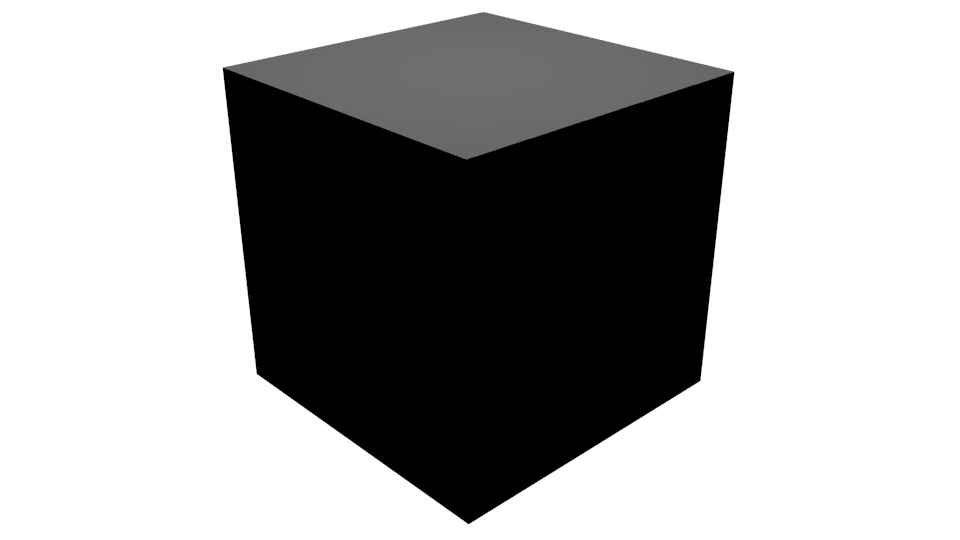
\includegraphics[width=\textwidth]{images/point.png}
%		\caption{Point}
%	\end{subfigure}
%	\begin{subfigure}{0.19\textwidth}
%		\centering
%		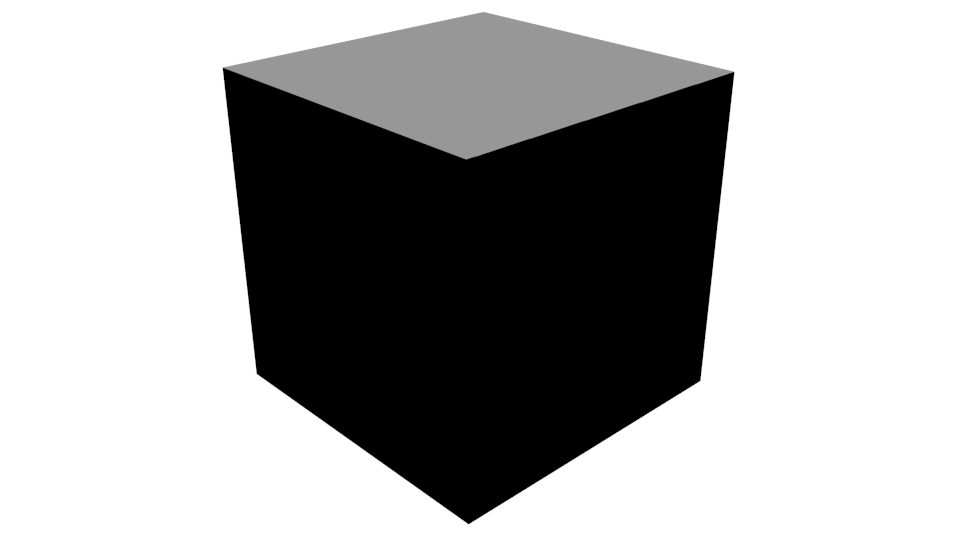
\includegraphics[width=\textwidth]{images/sun.png}
%		\caption{Sun}
%	\end{subfigure}
%	\begin{subfigure}{0.19\textwidth}
%		\centering
%		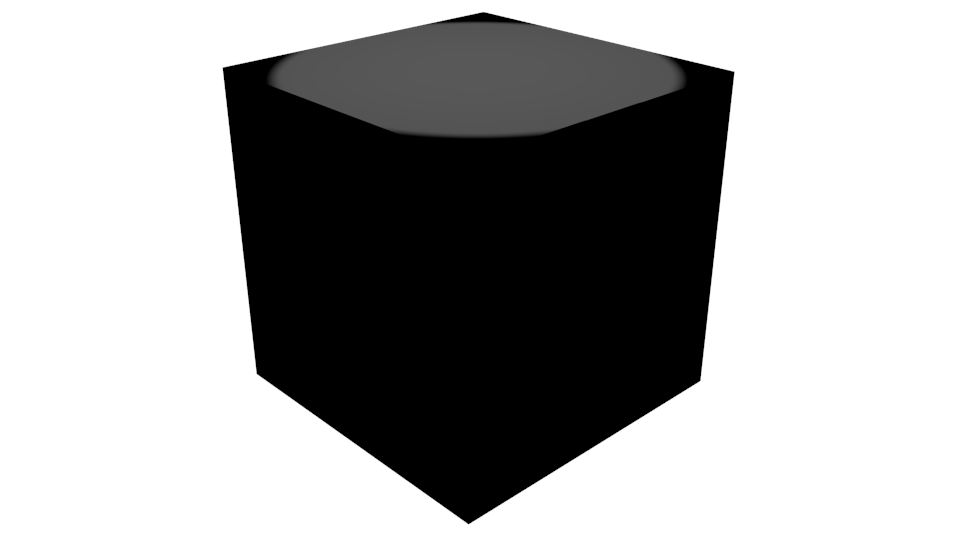
\includegraphics[width=\textwidth]{images/spot.png}
%		\caption{Spot}
%	\end{subfigure}
%	\begin{subfigure}{0.19\textwidth}
%		\centering
%		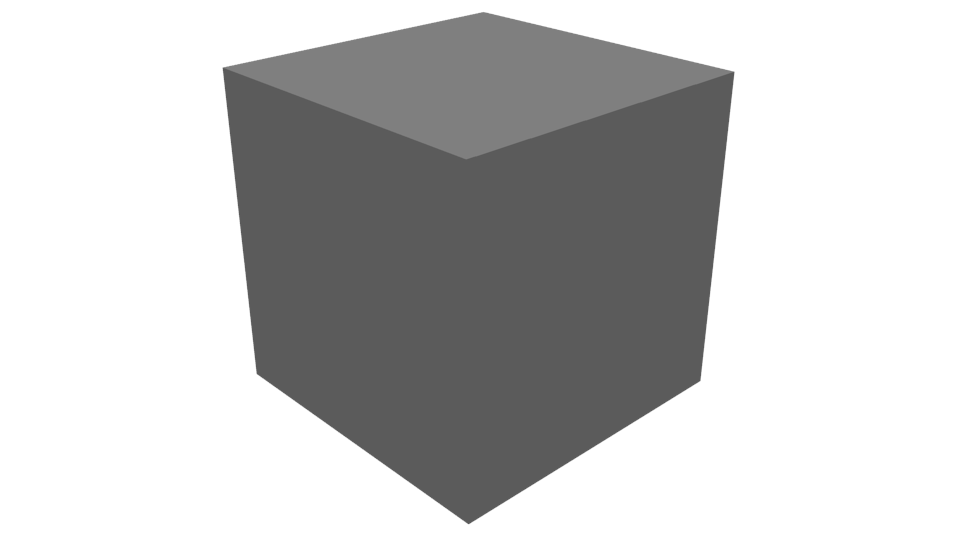
\includegraphics[width=\textwidth]{images/hemi.png}
%		\caption{Hemi}
%	\end{subfigure}
%	\begin{subfigure}{0.19\textwidth}
%		\centering
%		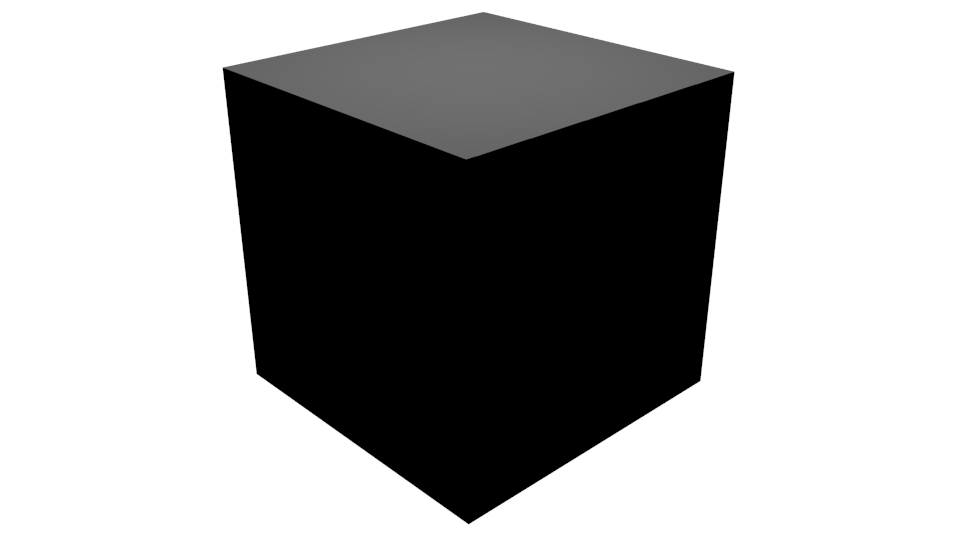
\includegraphics[width=\textwidth]{images/area.png}
%		\caption{Area}
%	\end{subfigure}
%	\caption[Lamp types available in Blender]{Lamp types available in Blender. Each light source is placed above the cube pointing directly towards it.}
%	\label{fig:blender-lamps}
%\end{figure}
Because all models have different heights and this type of lamp has no decay of intensity, it is placed above the objects far away from their origins.
By assigning the lamp a direction $\vec{r}_l = (0,0,0)^T$ it emits light along the negative $z$-axis directly onto the model.

For rendering views, a camera object is required.
Its parameters are left to the default values, except its view distance, which is set very high to work with all models.
Hence, only its location and rotation needs to be set.
Following the approach from \cite{Su:2015:MCN:2919332.2919750, Su2018} the camera is elevated 30 degrees from the ground plane and points towards the origin.
This results in the first rotation vector
\begin{equation}
	r_{c,0} = \left( \frac{r_{x,\text{deg}} \cdot \pi}{180}, 0, 0 \right)^T = \left( \frac{60 \cdot \pi}{180}, 0, 0 \right)^T
\end{equation}
in radians, where $r_{x,\text{deg}}$ is the rotation around the $x$-axis in degrees.
The first, second and third element define a rotation around the $x$-, $y$- and $z$-axis, respectively.
Because the camera points along the negative $z$-axis in its own coordinate system by default, $r_{x,\text{deg}} = 60$ corresponds to the mentioned setup.
The next step is fitting the camera view to the model just by changing the location of the camera.
Because Blender fits the camera view exactly to the object, an image padding is necessary for having empty border regions for later convolutions.
This is achieved by moving the camera away from the object along the line of their centers, i.\,e. along the negative view direction.
It is moved by
\begin{equation}
	\Delta d = \frac{d}{10}
\end{equation}
where $d$ is the distance from the mesh origin to the camera.
The advantage of a fraction is, that the padding is independent of the model's size.
Finally, this camera view is rendered with the following properties.
The resolution is defined to be $224 \times 224$ pixel
Furthermore, it needs to be coped with aliasing.
Because every pixel can only have a single color, diagonal lines usually have a step pattern.
This is not realistic, hence, it is smoothed out by anti-aliasing techniques.
This works by rendering the related image region in a higher resolution, taking several samples of pixel values and averaging them to get the value of the pixel in the desired resolution.
The best available sample size in Blender is 16, hence, it is chosen.
The background color is left at the default RGB color $\vec{c} = (64, 64, 64)$ resembling a dark gray for adding some noise to the views.
A black background would yield pixel intensities of 0 and resembles, in general, no real-world views.
Finally, this view is saved as a PNG file.
For gathering multiple views, the camera needs to be repositioned.
Hence, the following steps are repeated for the desired number of views.
The rotation of the camera is set to
\begin{equation}
	\vec{r}_c(v_i) = \left(  \frac{60 \cdot \pi}{180}, 0, \frac{v_i \cdot \varphi \cdot \pi}{180} \right)^T
\end{equation}
where $v_i$ is the view index, originally starting at 0, and $\varphi$ the moving interval in degrees.
The latter is set to
\begin{equation}
	\varphi = \frac{360}{n_v} = \frac{360}{12} = 30
\end{equation}
where $n_v$ equals the number of views.
For the ability to compare this work to related researches, $n_v = 12$ is defined.
The number of objects per set corresponds to \cite{Su:2015:MCN:2919332.2919750}.
That means, 90 objects per category class for the training set and 30 for the test set.
This process is repeated for each CAD object.